\chapter{Numerische Methoden}
\section{Einleitung}
\section{GPGPU Computing mit CUDA}
\section{Finite Differenzen Verfahren}
\section{Validierung}
\newpage

\chapter{Immersed Boundary Methoden}

\begin{figure}[!bp]
  \centering
  \subfloat[kartesisches Gitter]{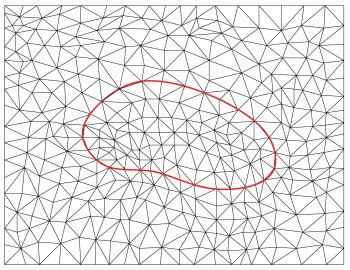
\includegraphics[width=0.4\textwidth]{gfx/immersed_boundary_methods/general_partition_triangle.jpg}\label{fig:f1}}
  \hfill
  \subfloat[unstrukturiertes Gitter]{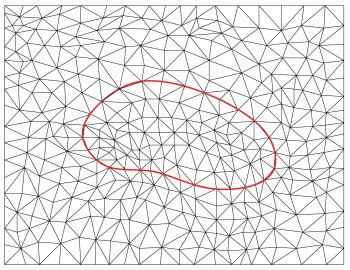
\includegraphics[width=0.4\textwidth]{gfx/immersed_boundary_methods/general_partition_triangle.jpg}\label{fig:f2}}
  \caption{Beispiele für numerische Gitter}
\end{figure}

\section{Einleitung}
Die bisher eingeführten Methoden eignen sich um auf einfachen Geometrien Simulationen durchzuführen.
Wenn die Ränder des Simulations-Gebietes nicht mehr mit dem numerischen Gitter übereinstimmen, lassen
sich die in Abschnitt () eingeführten Randbedingungen nicht mehr verwenden.
Das Problem lässt sich durch die Einführung eines an den Rand angepassten Gitter umgehen (s.Abb. \label{fig:f1}),
führt allerdings zu einem deutlich höheren Aufwand in den numerischen Berechnungen.
Die Berechnung des Gitters kann sehr aufwendig werden und es ist nicht eindeutig klar unter welchen
Performance-Einbussen sich das neue Gitter in der GPGPU-Implementierung verwenden lässt, da Bedingungen wie
z.B. Coalesced Readings  (s.Abbschnitt x) durch die unstrukturierten Daten deulich erschwert wären.
Eine Alternative die in dieser Arbeit verwendet wird sind  sog. Immersed Boundary Methoden.


- Beschreibung allgemein verschiedene immersed boundary methoden direkt /exp/ imp etc
    -erstmal peskin et al.
    -im prinzip 3 verschiedene ansätze continuous / direct /  ghost cell methoden
    - hier einfache methoden wegen gpu


\newpage

\section{No-Slip-Boundaries}
Für die unterschiedlichen Skalare in den Bousinnesqe gleichungen gibt es eine Vielzahl an möglichen Randbedingungen (s.Abbschnitt. X).
Während für die Geschwindigkeitsfelder häufig No- oder Free-Slip Ränder verwendet werden,
kommen bei der Temperatur oft NoFlux-Randbedingungen zum Einsatz um einen Wärmeaustausch mit der Umgebung zu unterdrücken.
Wie sich heraussgestellt hat ist die Implementierung von NoFlux-wänden mittels IBM wesentlich komplexer.
Die einzelnen Randbedingungen wurde daher getrennt voneinander untersucht, zunächst werden NoSlip-Ränder (s. gl. X) betrachtet.

\subsection{Volume Penalization}
Die Volume-Penalization Methode ermöglicht es, durch einen Kraftterm der auf die einzelnen Fluidzellen wirkt, mit wenig Aufwand Noslip-Ränder zu implementieren.
Das Verfahren wurde in mehreren Publikationen z.B. [bla] erfolgreich verwendet, eine mathematisch exaktere Abhandlung lässt sich z.B. in [bla2] finden.

\begin{wrapfigure}{r}{0.5\textwidth}
  \begin{center}
  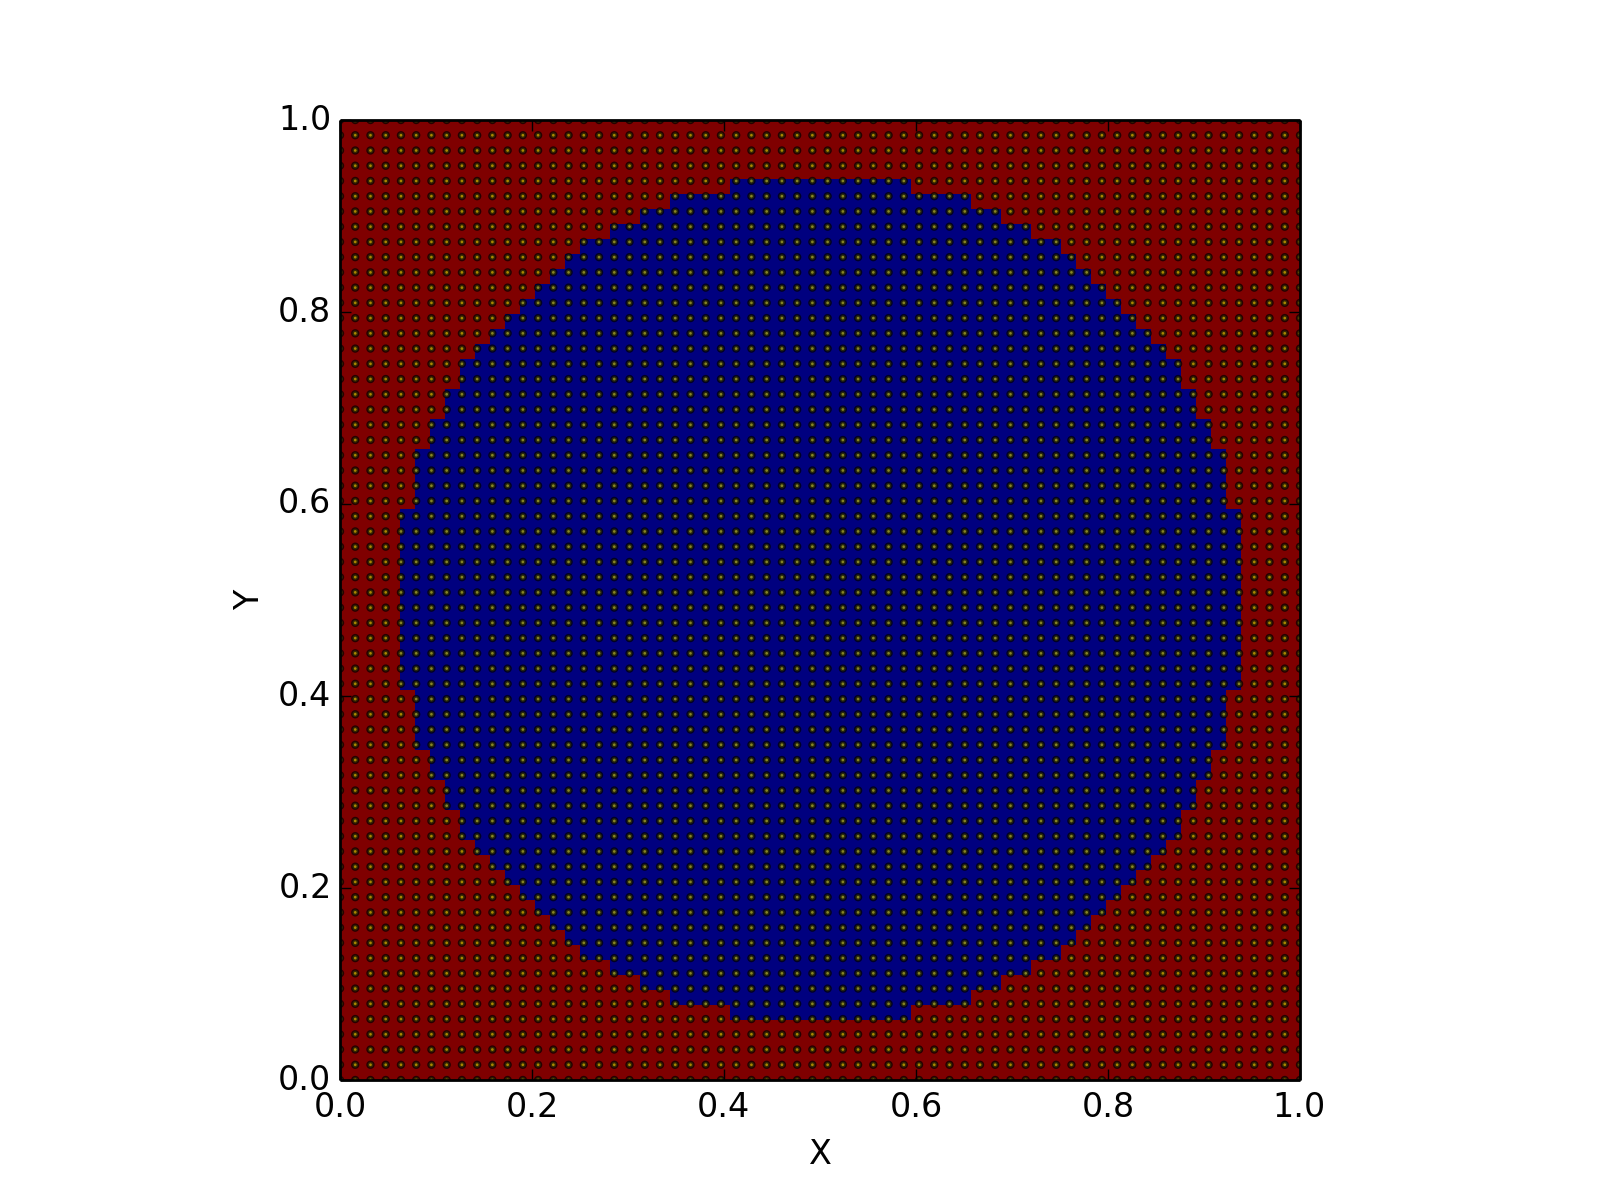
\includegraphics[width=0.5\textwidth]{gfx/immersed_boundary_methods/mask.png}\label{fig:mask_vp}
    \includegraphics[width=0.48\textwidth]{birds}
  \end{center}
  \caption{Maskierungsfunktion $H(x,y,z=const.) = x^2 + y^2 < c$ für einen Zylinder. }
\end{wrapfigure}

Das Volumen wird zunächst in einen Fluidbereich und einen festen Wandbereich, wie in Abb.1 dargestellt, unterteilt. Für die Differenzierung der Bereiche während der Simulation wird  eine Maskierungsfunktion
\begin{align}
H(x, y, z) = \begin{cases}
                    0, & \text{für } \vec{x}(x,y,z) \in Fluid, \\
                    1, & \text{sonst}.
             \end{cases}
\end{align}
verwendet. Als zusätzlicher Kraftterm wird nun eine exponentielle Dämpfung eingeführt die nur auf den Wandbereich des Volumens wirkt.
\begin{align}
\vec{f} = \frac{H(x, y, z)}{\nu}(\vec{v} - \vec{v_0})
\end{align}
Bei $\vec{v_0}$ handelt es sich um die gewünschte Randbedingung, der Kraftterm ist also proportional zur Auslenkung $\vec{v}$ eines Punktes vom gewünschten Ruhezustand.
Die Antwort des Kraftterms wird durch die Dämpfungrate $\nu$ reguliert. Je kleiner $\nu$ desto stärker ist die Dämpfungsrate, allerdings kann der Term
nicht beliebig klein gesetzt werden da die Stabilität für $\nu < dt$ nicht mehr gewährleistet ist [source].
Da für die Lösung der der Geschwindingskeitsfelder mit der Methode der künstliche Kompressibilität  bereits ein sehr kleiner Zeitschritt verwendet wird (s.Abb. X)
kann im Vergleich zu anderen Verfahren wie z.B. (pseudo-spektrale) eine relativ starke Dämpfungsrate verwendet werden.

\subsubsection{Validierung mit MASA}
-validierung mit masa für alle verfahren oben.. cube /evtl zylinder?
-vegl. und argumentation ränder ehh auf null.
-ein beispiel mit vol.pen.

\subsubsection{Validierung : planare Poiseuille Strömung}
Es stellt sich die Frage in welcher Größenordnung die Dämpfungskonstante $\nu$ der Volume Penalization methode liegen muss, um einen möglichst kleinen
Fehler zu gewährleisten. Ein einfacher Testfall der sich hierfür betrachen lässt ist eine einfache planare poiseuille strömung, diese ist schematisch in Abb. (x). dargestellt.
\paragraph*{Theoretische Beschreibung}\mbox{}\\
Wir betrachten eine laminare Strömung in x-Richtung die durch einen Druckgefälle $f=-\frac{\partial p}{\partial x}$ angetrieben wird.
Für die x- und y-Richtung werden periodische Randbedingungen angenommen. In z-Richtung wird das Volumen durch zwei Ebenen bei $h_1$ und $h_2$ begrenzt,
es gilt $\vec{v}(z=h_1) = \vec_{v}(z=h_2) = 0$.
Im stationären Fall lässt sich  die Bewegungsgleichung dann  auf eine Dimension reduzieren, es gilt:
\begin{align}
\frac{\partial v_x}{\partial t} &= - \frac{\partial p}{\partial x} + D \frac{\partial^2 v_x}{\partial z^2} = 0 \\
\Rightarrow v_x &= \frac{1}{2D}\frac{\partial p}{\partial x}z^2 + zc_1 + c_2\\
\end{align}
Mit $\vec{v}(h_1) = \vec_{v}(h_2) = 0$ und $A:=\frac{1}{2D}\frac{\partial p}{\partial x}$ ergibt sich:
\begin{align}
c_1 &= A\frac{h_1^2 -h_2^2}{h_2 - h_1} = -A(h_1+h_2)\\
c_2 &= A(h_1(h_1 + h_2) - h_1^2) = Ah_1h_2\\
\Rightarrow v_x &= A(z^2 - z(h_1 + h_2) + h_1h_2)
\end{align}
Da die Strömung in der Kanalmitte am stärksten ist gilt zudem:
\begin{align}
z_{max} &= \frac{h_1+h_2}{2}\Rightarrow v_{max} = A\left(h_1h_2 - \frac{(h_1 + h_2)^2}{4}\right)
\end{align}
Für die Strömung lässt sich die Reynoldszahl dann gemäß $Re \propto \frac{v_{max}}{D}$  bestimmen.

\paragraph*{Setup}\mbox{}\\
Um die Abhängigkeit des Fehlers von der Dämpfungskonstante zu betrachten wurde ein Kanal mit $l_x=1$, $l_y=1$ und $l_z=2$ sowie $h_1=0.25$, $h_2=0.75$.
betrachtet. Die Maskierungsfunction ergibt sich damit gemäß $H(z) = (z>h1) & (z<h2)$.
Für die Reynoldszahl wurden Werte im Intervall $Re \in [100, 500]$ verwendet, die Dämpfungskonstante wurde zwischen $\nu \in [1e-5, 0.1]$ variert, während der Zeitschritt mit $dt =1e-5$ konstant gehalten wurde. Die genauen Angaben für alle Parameter sind in (Anhang Tab.X) zu finden.

\paragraph*{Ergebnisse}\mbox{}\\
Zunächst ist in Abb.X das Geschwindigkeitsprofil der Strömung für $Re=X$ dargstellt. Es lässt sich bereits qualitativ sehr gut erkennen, dass für eine
starke Dämfung die Kanalströmung an den Grenzen $h_1$ und $h_2$ verschwindet. Je kleiner Die Dämpfungrate ist desto stärker entwickelt
sich im Rand ein Geschwindigkeitsprofil. Um sicherzustellen dass sich das Profil vollständig entwickelt hat wurde die Simulation bis zu dem
Zeitpunkt fortgegeführt in welchem die kinetische Energie einen stationären Wert erreicht, s.Abb.X(b).


\begin{figure}[!bp]
  \centering
  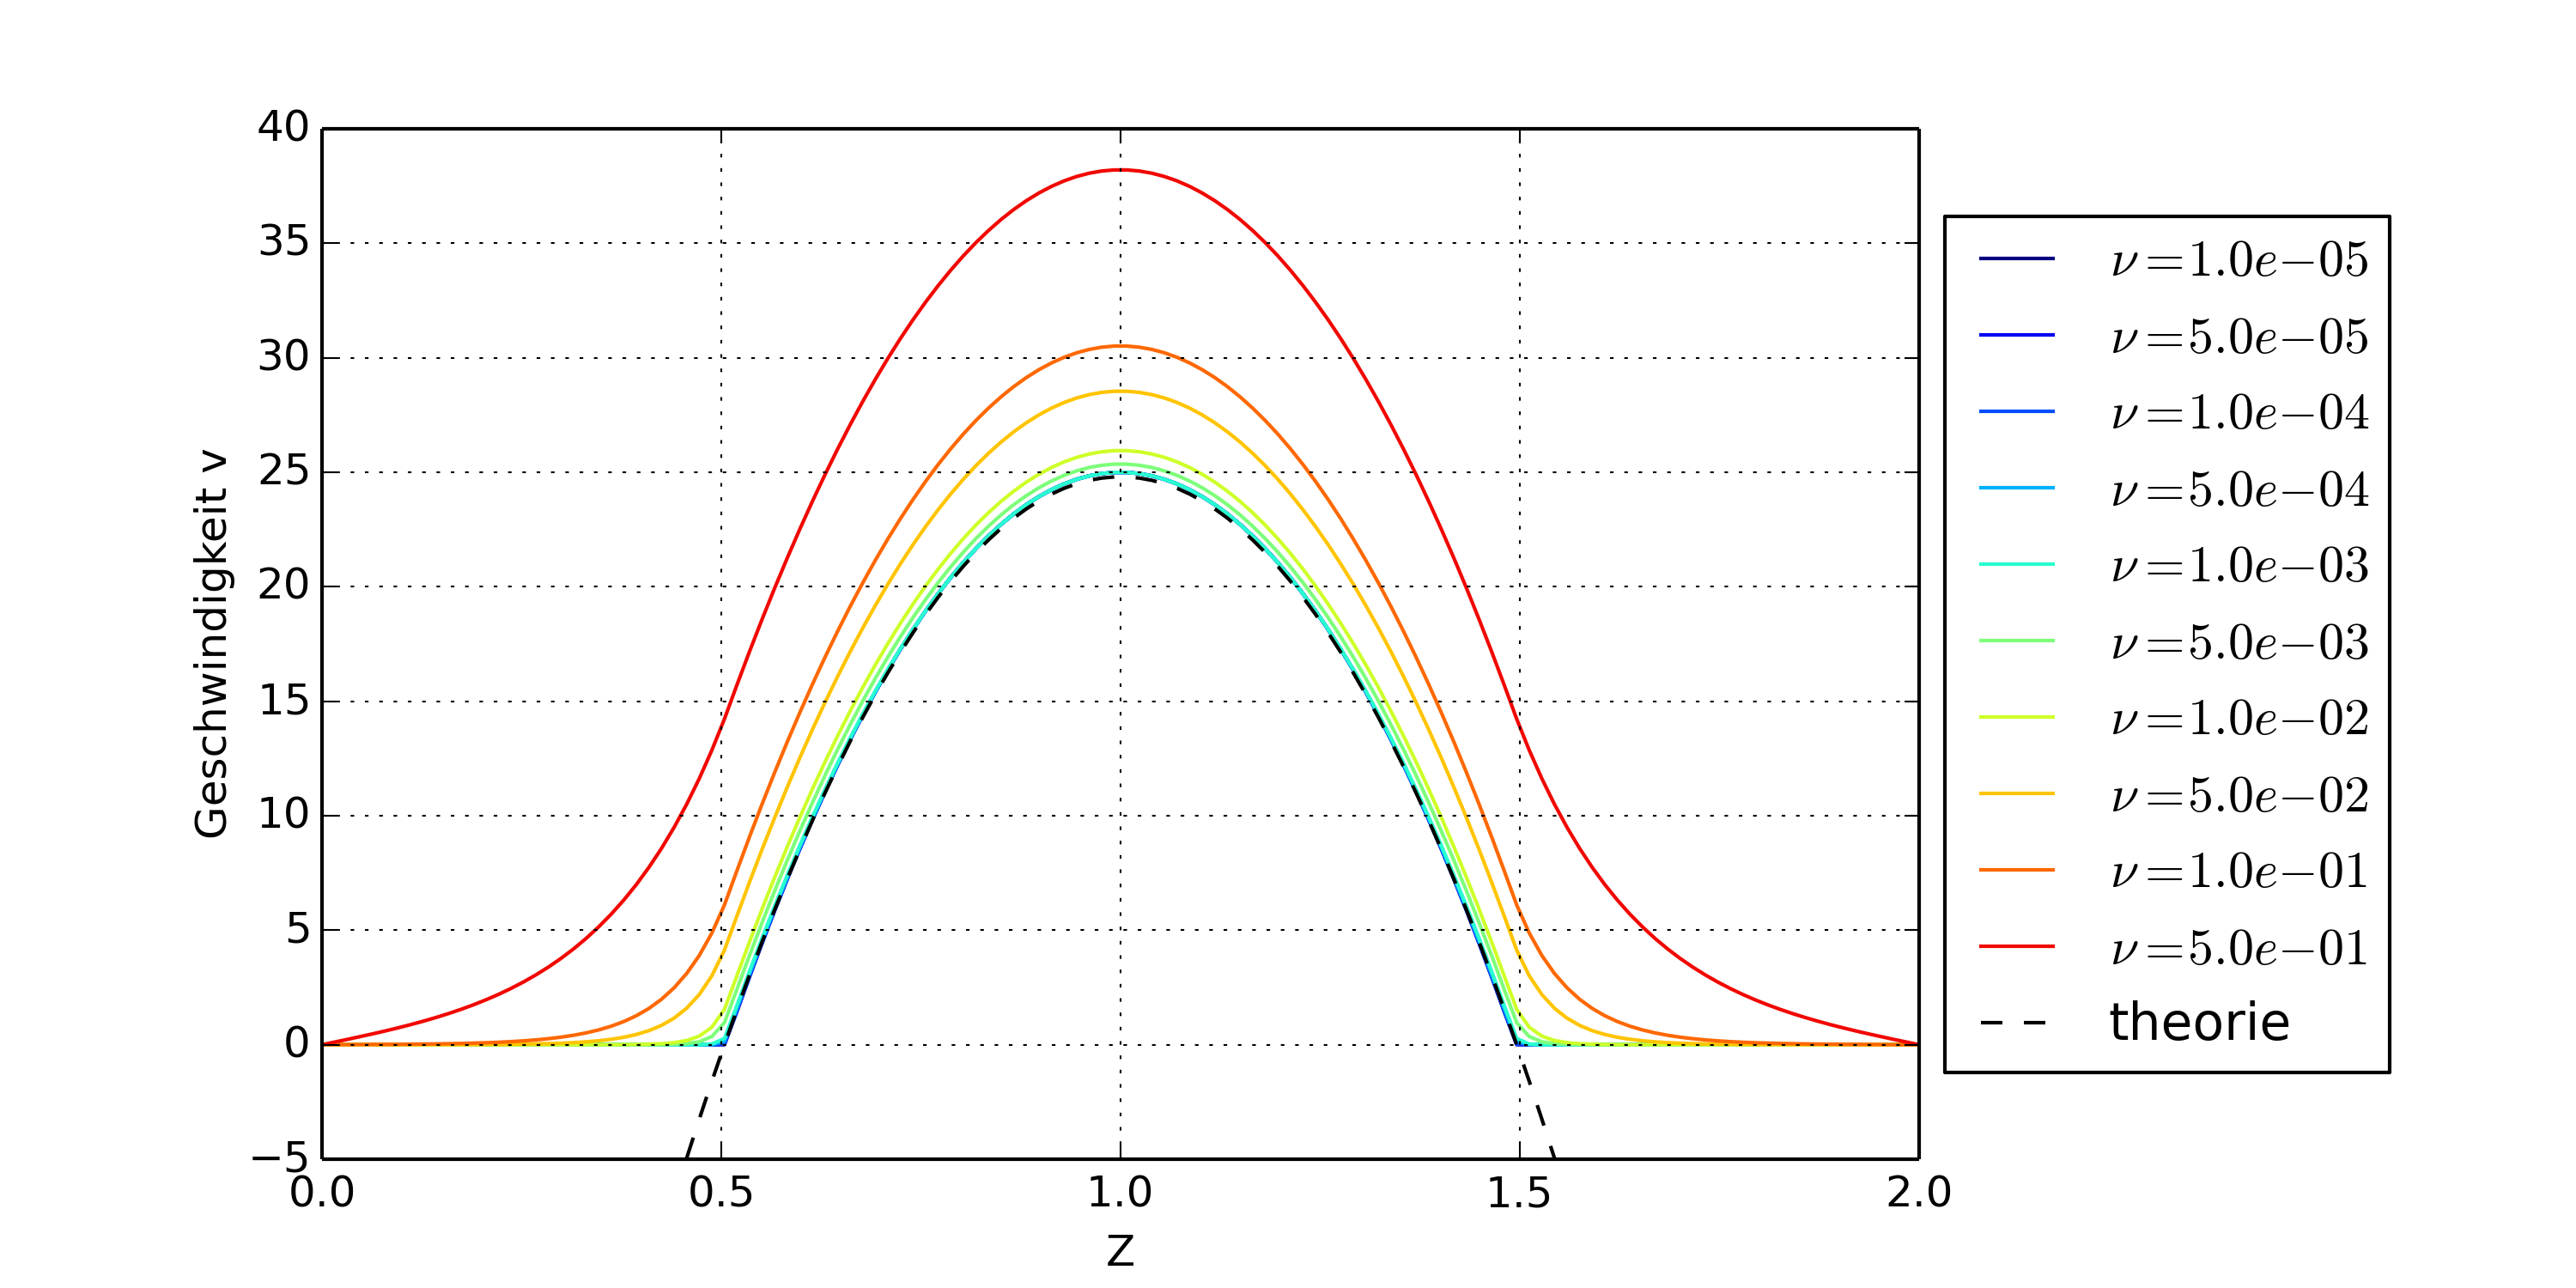
\includegraphics[width=1.0\textwidth]{gfx/immersed_boundary_methods/vp_flow.png}\label{fig:f4}
  \caption{Beispiele für numerische Gitter}
\end{figure}



-plot beispiel flow
-plot fehler gegen nu
-streifen diskussion
-blabla



\subsection{Direct Forcing}
-Paper quote
-vgl volume penalization warum keine instablilität
-formeln
-implementierung

\subsection{Direct Forcing mit Volume Fraction}
-paper quote formeln
-implementierung beispiel

\section{Direct Forcing mit Interpolation}
-paper quote formeln
-implementierung beispiel

\section{Methoden-Vergleich und numerische Validierung}
In diesem Abschnitt sollen die verschiedenen Methoden über numerische Testfälle validiert und miteinnander
verglichen werden.


\subsubsection{Poiseuille Strömung im Zylinder}

\subsubsection{Zusammenfassung}


\subsection{No-Flux-Boundaries}

\subsubsection{'Variable Konduktivität'}










